\chapter{Photonic Reservoir Computer with Wavelength Division Multiplexed neurons}

\label{ch-wdm-rc}

In this chapter, a novel approach of \gls{prc} is proposed, in which the neurons are no longer multiplexed in time, but in wavelength (or frequency) instead. This scheme was introduced in \cite{AkroutAkram2016Pprc} and its end goal is to overcome the speed limitations imposed by the \gls{tdm} of the neurons, as exposed in section \ref{tdm-neurons-principle}. Indeed, by multiplexing the neurons in the frequency domain, the input signal can reach them all in the same time, there is no need to slow down its pace to let it alter the neurons sequentially. As an illustration, in \cite{Vandoorne2014}, they proposed the first \gls{prc} with parallelisation of the neurons. In the experiment described in the paper, the neurons were spatially multiplexed. Doing so, the authors were able to reach data processing rates up to 12.5 GHz on tasks such as header recognition or boolean logic, which is an increase of one order of magnitude compared to those reported in \cite{Vinckier2015}. This is encouraging for research in parallel \gls{prc} and motivates the study of the scheme explored in this thesis.\\

First, in section \ref{sec-scheme-wdm}, a description of the working principle is given. It starts with a high-level overview of the scheme in which different features and components are presented. After that, attention is brought to the frequency coupling mechanism used to let the neurons interact between one another. It is shown that this can be achieved using a optoelectronic \gls{pm}, even though this device has some practical drawbacks. Finally, the scheme is described with more details. In section \ref{sec-challenges-wdm}, the stabilisation issue, which is main topic of this thesis, is introduced.

%%%%%%%%%% DESCRIPTION OF THE SCHEME %%%%%%%%%%

\section{Description of the scheme}

\label{sec-scheme-wdm}

In this section, the working principle of \gls{wdm} \gls{prc} is first given. This scheme takes advantage of the wave character of light and uses different wavelength to encode the neurons. It is fibre-based and relies on an optical cavity made of a fibre loop. Inside the resonator, the different neurons need to be able to interact, therefore one has to provide some coupling mechanism for the different frequencies. This issue is tackled in section \ref{subsec-freq-coupling} and provides interesting mathematical insights that are eventually used to derive a suitable model for this other kind of linear \rcer.

%%% WORKING PRINCIPLE %%%

\subsection{Working principle}

The working principle of the new reservoir is schematised on figure \ref{wdm_rc_principle}. The whole setup is fibre-based, and the fibre used is a polarisation maintaining, single mode fibre. 

\paragraph{Input}

The input time series $u(n)$ is converted into a continuous signal $\tilde{u}(t)$ by keeping its value constant during one period $\tau$ (sample and hold procedure), which leads to $\tilde{u}(t)=u(n)$, with $t \in [n\tau, (n+1)\tau[$. The continuous, coherent light emitted by a narrow band laser at frequency $\omega_0$ is modulated in intensity by the input signal $\tilde{u}(t)$ using a \gls{mzm}.  

\paragraph{Cavity}

The modulated data is then coupled to an optical cavity around 20 metres long\footnote{The length of the cavity can be derived from its \gls{fsr}, which is studied in the next chapter}. Inside this cavity, a \gls{pm} mixes the different optical frequencies. More information about the \gls{pm} can be found in section \ref{subsec-freq-coupling}. Losses are introduced inside the cavity by two main sources, the intrinsic losses of the fibre and the insertion losses of the \gls{pm}, hence the presence of an intra-cavity amplifier used to compensate for them. The neurons are encoded in the electric field evolving inside this cavity, which is schematised on the figure by the three different colours for the fibre loops. Therefore, from now on, the cavity is referred to as the \textit{reservoir}. The holding time $\tau$ introduced earlier should be equal to the \gls{rtt} of the reservoir. This is done in order to update the discrete dynamics of the \rcer each time the light completes a trip around the cavity. Doing so, one ensures that the value of the neuron $x_j$ at discrete time $n+1$ depends on the values of the neurons $x_i$, with $i \in \{1,\dots, N\}$, at precisely time $n$. 

\paragraph{Readout}

The electric field encoding the neurons exits the cavity through another coupler, and is then demultiplexed in frequency. Each of the frequency component is measured using a \gls{pd}, which gives a value proportional to the squared modulus of the electric field, as explained in the previous chapter. The resulting signals are linearly combined using the trained output weights to produce the output of the reservoir $y(n)$.

\begin{equation}
	y(n) = \sum_{i=1}^{N} W_i^{\text{out}} |x_i(n)|^2
\end{equation}

\begin{figure}[h]
	\centering
	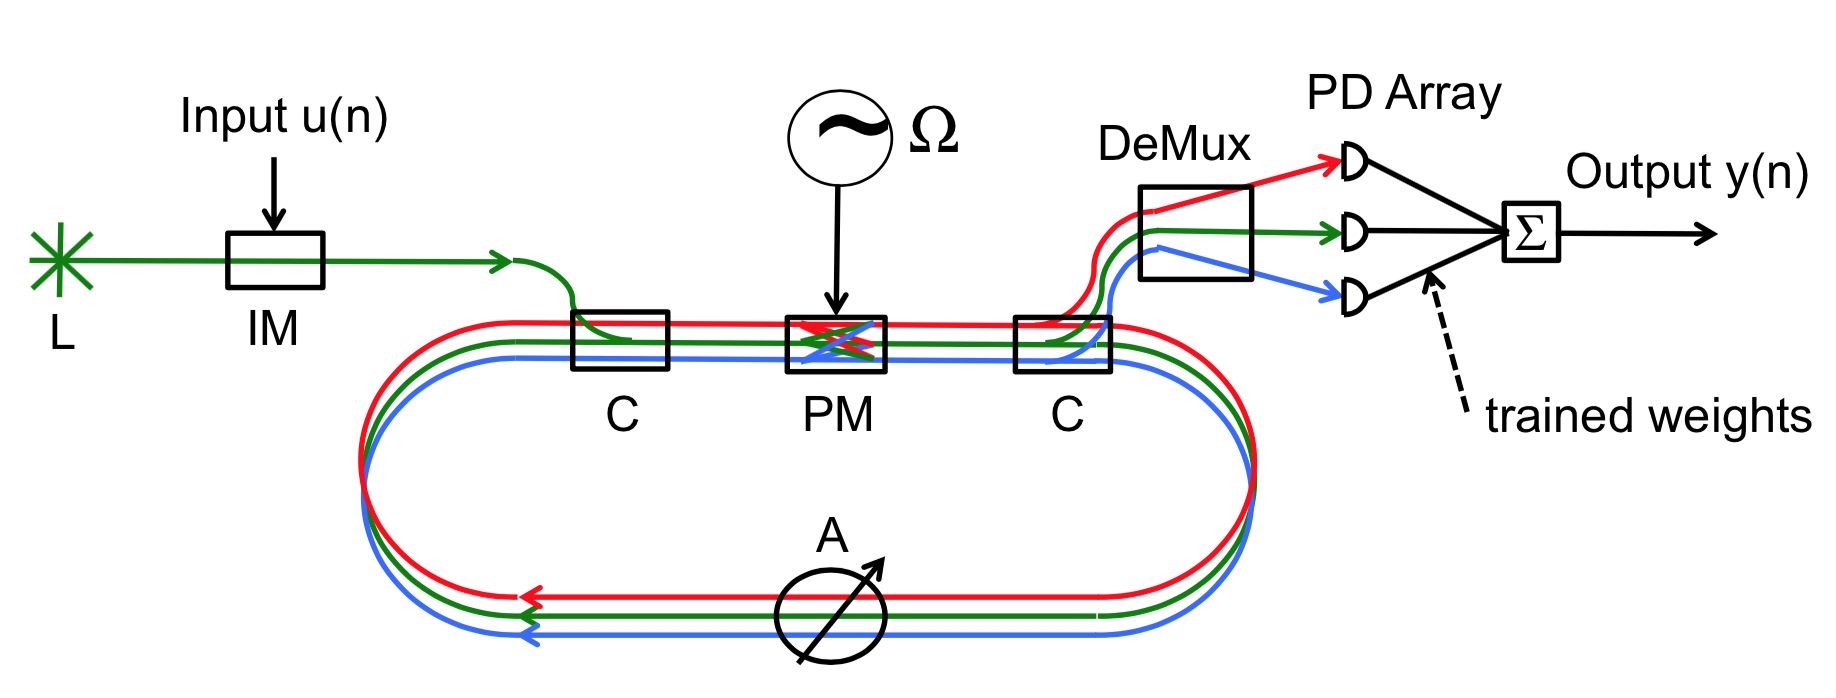
\includegraphics[width=\textwidth]{wdm_rc_principle}
	\caption{Schematic representation of the working principle of the \gls{wdm} \gls{prc} \cite{AkroutAkram2016Pprc}}
	\label{wdm_rc_principle}
\end{figure}

\paragraph{Training and testing}

The training scheme used for this setup is the batch learning. Thus, to compute the output weights $\wout$, one can use the ridge regression technique introduced in section \ref{subsec-rc-training}. To do so, one needs to discard the first state vectors $\mathbf{x}$ because they correspond to the transient of the reservoir, and then to store them\footnote{Since the output $y$ is constructed using the squared modulus of the activation of the neurons, the matrix $\mathbf{X}$ is filled with $|x_i(n)|^2$ instead of what is indicated in section \ref{subsec-rc-training}, namely $x_i(n)$} as well as the desired outputs $\hat{y}$ during the whole learning period to create the matrices $\mathbf{X}$ and $\hat{\mathbf{Y}}$. After that, it is straightforward to solve equation \eqref{ridge-regression} and to find the output weights. Once the \rcer is trained, it can move on to the testing phase, during which the outputs $y(n)$ are compared to the desired outputs. From that, one can quantify the performance of the \rcer using the appropriate metric, such as the \gls{nmse} for example.

%%% FREQUENCY COUPLING OF THE NEURONS %%%

\subsection{Frequency coupling of the neurons}

\label{subsec-freq-coupling}

To mix the different frequencies present inside the reservoir a \gls{pm} is used. This kind of device is well known for creating equidistant sidebands. Let $Ee^{i\omega t}$ be the input electric field entering the \gls{pm}. Since a \gls{pm} is an optoelectronic device, it needs to be externally driven by a voltage generator with a RF modulation signal $V_{\text{RF}}(t) = A \sin{(\Omega t)}$, with $\Omega \ll \omega$. Using the \textit{Anger-Jacobi} expansion that allows to express the exponential of a trigonometric function in the basis of its harmonics, one can express the effect of a \gls{pm}:

\begin{align}
	&Ee^{i\omega t} \overset{\Omega}{\longrightarrow} Ee^{i\omega t}e^{im\sin{(\Omega t)}} \nonumber \\
	& = E \sum_{n=-\infty}^{\infty} J_n(m) e^{i(\omega+n\Omega)t} \label{tf-pm}
\end{align}

This formula indicates that the resulting wave is a discrete superposition of planar waves whose frequencies are evenly spaced ($\pulsefreq{\Omega}$ between each frequency component) and centred on the input electric field frequency $\pulsefreq{\omega}$. The coefficient $J_n(m)$ weighting the superposition is the $n^{\text{th}}$ order Bessel function and $m$ is the modulation depth. The latter is related to the modulation amplitude $A$, but the link between them is not straightforward and is experimentally investigated in the next chapter. 

\begin{figure}[h]
	\centering
	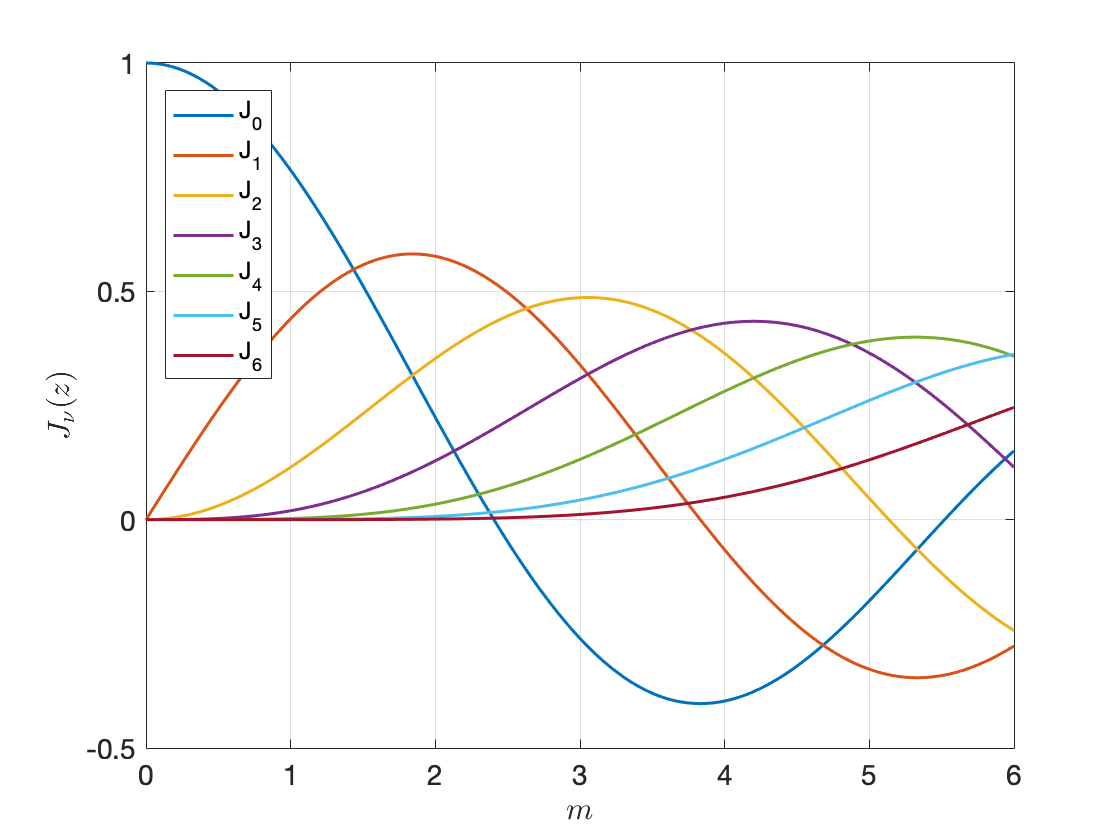
\includegraphics[width=.6\textwidth]{bessel}
	\caption{Bessel function of order $n \in \{0,\dots,6\}$}
	\label{bessel}
\end{figure}

However, what can already be said about $m$ is that it cannot exceed 2 in practice. This is due to the fact that when one increases the modulation frequency $\pulsefreq{\Omega}$, the modulation amplitude $A$ cannot be brought to arbitrarily large values. As a first approximation regarding the RF generator, one could say that the product $\Omega A$ is upper bounded. On figure \ref{bessel}, one can observe the behaviour the Bessel functions $J_n(m)$ with $n \in \{0,\dots, 6\}$. For $m \in [0,2]$, $J_n(m)$ becomes less significant for increasing order $n$. This provides an insight on an intrinsic limitation of this kind of \rcer, which is the limited number of neurons. A possible solution to improve the scheme would be to use a longitudinal multimode laser\footnote{A longitudinal multimode laser emits light at different frequencies} to inject energy in a wider range of neurons. Yet, the coupling between distant neurons would still be very faint.

\begin{figure}[h]
	\centering
	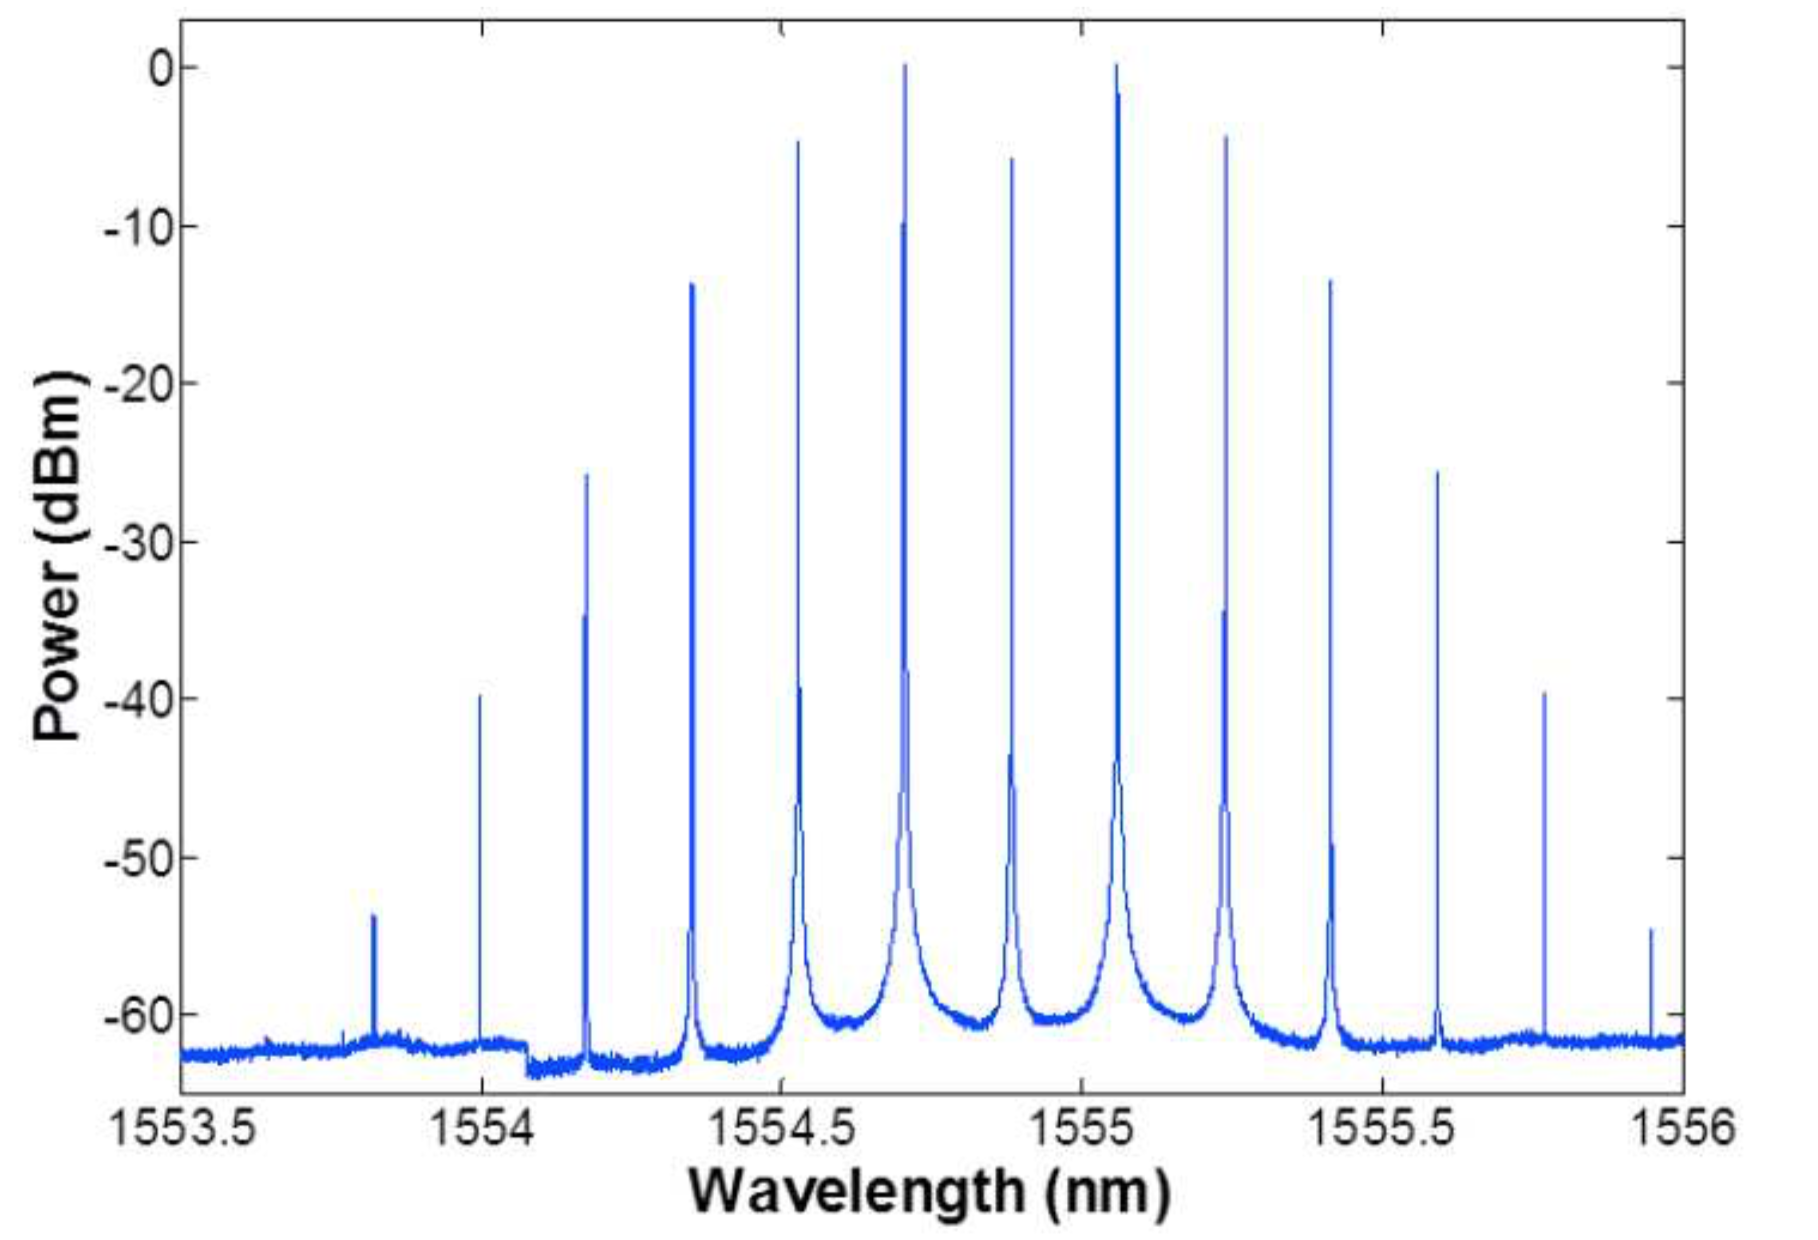
\includegraphics[width=.7\textwidth]{power-in-neurons}
	\caption{Experimental spectral density inside the reservoir \cite{AkroutAkram2016Pprc}}
	\label{power-in-neurons}
\end{figure}

On figure \ref{power-in-neurons}, the elements regarding the fast decrease of the intensity of the sidebands brought to light in the previous paragraph are confirmed experimentally. On this graph, one can see that only 13 neurons are usable in practice. One also notices that the spectrum is symmetric with respect to the central neuron. This can be explained by the fact that the height of the $n^{\text{th}}$ peak is $\propto |J_n(m)|^2$, and by using a property of the Bessel functions that says that for $n \in \mathbb{Z}$, $J_{-n}(m)=(-1)^n J_n(m)$:

\begin{equation}
	|J_{-n}(m)|^2 = |(-1)^n J_n(m)|^2 = |J_n(m)|^2
\end{equation}

%%% MATHEMATICAL MODEL %%%

\subsection{Mathematical model}

This section tackles the derivation of the discrete equation governing the dynamics of the reservoir. This calculation relies on the result stemming from the previous section regarding the effect of a \gls{pm} on an incident electric field. As a first step, the state $\mathbf{x}$ is expressed using a convenient formalism. The end goal here is to be able to use linear algebra because it makes the derivation easier. Let $N$ be the total number of neurons. This implies that $\mathbf{x}$ should be a $N$-dimensional vector that can developed as a linear combination of basis vectors:

\begin{equation}
	\mathbf{x} = \sum_{i=1}^{N} x_i \hat{\mathbf{e}}_i
\end{equation}

If the basis vectors are adequately chosen, the state vector $\mathbf{x}$ can reduce to the value of the electric field inside the reservoir. The basis vectors are defined as:

\begin{equation}
	\hat{\mathbf{e}}_n = e^{i\omega_nt} = e^{i(\omega+n\Omega)t}
\end{equation}

Moreover, to be consistent, the numbering of the neurons should be modified such that $\hat{\mathbf{e}}_0$ corresponds to the central frequency. Let $\eta$ be the new variable used to iterate through the neurons such that the sum in the linear combination will go from $-\eta$ to $\eta$ instead of from 1 to $N$. $\eta$ is given by $\lfloor N/2 \rfloor$. The state vector $\mathbf{x}$ now reads:

\begin{equation}
	\mathbf{x} = \sum_{i=-\eta}^{\eta} x_i \hat{\mathbf{e}}_i
\end{equation}

This is precisely equal to the electric field inside the reservoir. The results from the previous section con now be used to derive the discrete dynamics equation. Knowing the value of each of the neurons at discrete time $n$ and the effect of a \gls{pm}, one can compute the new state vector. To do so, linear algebra is used. One knows that the reservoir is linear, therefore, it should be possible to find a linear mapping between two successive states. If there exists a linear mapping, since one is working in discrete space, there is a matrix representation of this mapping. Furthermore, given that one knows the effect of a \gls{pm} on each of the basis vectors, one can explicitly define this matrix.

\begin{equation}
	\mathbf{J} = \begin{bmatrix}
		J_0(m) & J_{-1}(m) & \dots & J_{-\eta}(m) & \dots & J_{-2\eta} \\
		J_1(m) & J_0(m) & \dots & J_{-\eta+1}(m) & \dots & J_{-2\eta+1} \\
		\vdots & \vdots &  & \vdots &  & \vdots \\
		J_{2\eta}(m) & J_{2\eta-1}(m) & \dots & J_\eta(m) & \dots & J_0
	\end{bmatrix}
\end{equation}

One should note that each time the light goes around the cavity, it acquires some phase which is dependent on the wavelength. This should be taken into account in the derivation as well. If $\phi_i$ is the phase acquired by the neuron propagating with the frequency $\pulsefreq{\omega_i}$, one can define the phase matrix:

\begin{equation}
	\mathbf{\Phi} = \begin{bmatrix}
		e^{i\phi_{-\eta}} & 0 & \dots & \dots & \dots & 0 \\
		0 & e^{i\phi_{-\eta+1}} & 0 & \dots & \dots & 0 \\
		\vdots & 0 & \ddots & & & \vdots \\
		\vdots & \vdots & & e^{i\phi_i} & & \vdots \\
		\vdots & \vdots & & & \ddots & 0 \\
		0 & 0 & \dots & \dots & 0 & e^{i\phi_{\eta}}
	\end{bmatrix}
\end{equation}

Both $\mathbf{J}$ and $\mathbf{\Phi}$ are $N\times N$ matrices. Finally, recalling that $\alpha$ and $\beta$ are the feedback and input gains, respectively, and that the source laser only injects in the central wavelength, one can express the discrete time dynamics of the reservoir:

\begin{equation}
	\mathbf{x}(n+1) = \alpha \mathbf{\Phi} \mathbf{J} \mathbf{x}(n) + \beta u(n+1) \hat{\mathbf{e}}_0
\end{equation}

A few things need to be mentioned. The value of $\alpha$ can be adjusted experimentally by changing the intra-cavity amplification and that of $\beta$ numerically in the computer controlling the experiment. Finally, to be consistent with the model derived here, the figure \ref{wdm_rc_principle}, coming directly from \cite{AkroutAkram2016Pprc}, should be slightly modified. Indeed, the \gls{pm} should be positioned before the input coupler and not between the input and readout coupler, because according to the figure, there should be no inhomogeneous term corresponding to the input signal.

%%%%%%%%%% CHALLENGES %%%%%%%%%%

\section{Challenges}

\label{sec-challenges-wdm}

% Stabilisation
% Stabilisation signal is the same as data signal











